% answers.tex —— 2009 年·普通高等学校招生考试·辽宁卷·文科 · 参考答案与详细解析片段
% 由 tools/generate_projects.py 依来源总账自 2009/2009_数学真题_辽宁文_试题.md + 2009/2009_数学真题_辽宁文_解析正文.md + 2009/2009_数学真题_辽宁文_答案要点.md 生成，勿手改（改源 MD 后重跑）


\begin{gktip}
固定候选 PDF 仅含题面，无答案、解析和评分标准，原卷亦未标分值；以下为非官方编者独立推导，官方答案字段为空。题面文字层只作定位，分数、根号、上下标与六幅图均以 600 dpi 原页复核。
\end{gktip}

\begin{answer}
\gksolhead{1}{}

\textbf{题目}：

已知集合 $M=\{x\mid -3<x\leqslant5\}$，$N=\{x\mid x<-5$ 或 $x>5\}$，则 $M\cup N=$（　）

（A）$\{x\mid x<-5$ 或 $x>-3\}$

（B）$\{x\mid -5<x<5\}$

（C）$\{x\mid -3<x<5\}$

（D）$\{x\mid x<-3$ 或 $x>5\}$

\Needspace{4\baselineskip}
\textbf{解析}

$M$ 是左开右闭区间 $(-3,5]$，$N$ 是两条射线 $(-\infty,-5)\cup(5,+\infty)$。取并集时注意 $5\in M$，故 $(-\infty,-5)\cup(-3,5]\cup(5,+\infty)=(-\infty,-5)\cup(-3,+\infty)$，即 $\{x\mid x<-5\ \text{\text{或}}\ x>-3\}$，选 A。

\gkanswer{答案：A。}

\end{answer}
\begin{answer}
\gksolhead{2}{}

\textbf{题目}：

已知复数 $z=1-2\mathrm i$，那么 $\frac1z=$（　）

（A）$\frac{\sqrt5}{5}+\frac{2\sqrt5}{5}\mathrm i$

（B）$\frac{\sqrt5}{5}-\frac{2\sqrt5}{5}\mathrm i$

（C）$\frac15+\frac25\mathrm i$

（D）$\frac15-\frac25\mathrm i$

\Needspace{4\baselineskip}
\textbf{解析}

\nopagebreak[4]
\[\frac1z=\frac{1}{1-2\mathrm i}
=\frac{1+2\mathrm i}{(1-2\mathrm i)(1+2\mathrm i)}
=\frac{1+2\mathrm i}{1+4}
=\frac15+\frac25\mathrm i,\]

选 C。

\gkanswer{答案：C。}

\end{answer}
\begin{answer}
\gksolhead{3}{}

\textbf{题目}：

$\{a_n\}$ 为等差数列，且 $a_7-2a_4=-1$，$a_3=0$，则公差 $d=$（　）

（A）$-2$

（B）$-\frac12$

（C）$\frac12$

（D）$2$

\Needspace{4\baselineskip}
\textbf{解析}

$a_7=a_3+4d=4d$，$a_4=a_3+d=d$，代入 $a_7-2a_4=-1$ 得 $2d=-1$，故 $d=-\dfrac12$，选 B。

\gkanswer{答案：B。}

\end{answer}
\begin{answer}
\gksolhead{4}{}

\textbf{题目}：

平面向量 $\boldsymbol a$ 与 $\boldsymbol b$ 的夹角为 $60^\circ$，$\boldsymbol a=(2,0)$，$|\boldsymbol b|=1$，则 $|\boldsymbol a+2\boldsymbol b|=$（　）

（A）$\sqrt3$

（B）$2\sqrt3$

（C）$4$

（D）$12$

\Needspace{4\baselineskip}
\textbf{解析}

\Needspace{5\baselineskip}
$\boldsymbol a\cdot\boldsymbol b=|\boldsymbol a||\boldsymbol b|\cos60^\circ=2\times1\times\dfrac12=1$。于是

\nopagebreak[4]
\[|\boldsymbol a+2\boldsymbol b|^2=|\boldsymbol a|^2+4\boldsymbol a\cdot\boldsymbol b+4|\boldsymbol b|^2
=4+4+4=12,\]

$|\boldsymbol a+2\boldsymbol b|=2\sqrt3$，选 B。

\gkanswer{答案：B。}

\end{answer}
\begin{answer}
\gksolhead{5}{}

\textbf{题目}：

如果把地球看成一个球体，则地球上北纬 $60^\circ$ 纬线长和赤道线长的比值为（　）

（A）$0.8$

（B）$0.75$

（C）$0.5$

（D）$0.25$

\Needspace{4\baselineskip}
\textbf{解析}

\Needspace{5\baselineskip}
北纬 $60^\circ$ 纬线是半径 $r=R\cos60^\circ=\dfrac R2$ 的小圆，其周长与赤道周长之比为

\nopagebreak[4]
\[\frac{2\pi r}{2\pi R}=\cos60^\circ=\frac12,\]

选 C。

\gkanswer{答案：C。}

\end{answer}
\begin{answer}
\gksolhead{6}{}

\textbf{题目}：

已知函数 $f(x)$ 满足：当 $x\geqslant4$ 时，$f(x)=\left(\frac12\right)^x$；当 $x<4$ 时，$f(x)=f(x+1)$．则 $f(2+\log_23)=$（　）

（A）$\frac{1}{24}$

（B）$\frac{1}{12}$

（C）$\frac18$

（D）$\frac38$

\Needspace{4\baselineskip}
\textbf{解析}

\Needspace{5\baselineskip}
$2+\log_23\in(3,4)$，先按 $x<4$ 的递推式：

\nopagebreak[4]
\[f(2+\log_23)=f(3+\log_23),\]

\Needspace{5\baselineskip}
而 $3+\log_23>4$，故直接用第一段解析式：

\nopagebreak[4]
\[f(3+\log_23)=\left(\frac12\right)^{3+\log_23}
=\left(\frac12\right)^3\cdot\left(\frac12\right)^{\log_23}
=\frac18\cdot\frac13=\frac1{24},\]

选 A。

\gkanswer{答案：A。}

\end{answer}
\begin{answer}
\gksolhead{7}{}

\textbf{题目}：

已知圆 $C$ 与直线 $x-y=0$ 及 $x-y-4=0$ 都相切，圆心在直线 $x+y=0$ 上，则圆 $C$ 的方程为（　）

（A）$(x+1)^2+(y-1)^2=2$

（B）$(x-1)^2+(y+1)^2=2$

（C）$(x-1)^2+(y-1)^2=2$

（D）$(x+1)^2+(y+1)^2=2$

\Needspace{4\baselineskip}
\textbf{解析}

\Needspace{5\baselineskip}
两条平行线 $x-y=0$ 与 $x-y-4=0$ 之间的距离为

\nopagebreak[4]
\[d=\frac{|0-(-4)|}{\sqrt{1^2+(-1)^2}}=\frac4{\sqrt2}=2\sqrt2,\]

圆与两线都相切，故半径 $r=\dfrac d2=\sqrt2$。圆心到两线距离相等，位于中位线 $x-y-2=0$ 上；又圆心在 $x+y=0$ 上，联立得圆心 $(1,-1)$。所求方程为 $(x-1)^2+(y+1)^2=2$，选 B。

\gkanswer{答案：B。}

\end{answer}
\begin{answer}
\gksolhead{8}{}

\textbf{题目}：

已知 $\tan\theta=2$，则 $\sin^2\theta+\sin\theta\cos\theta-2\cos^2\theta=$（　）

（A）$-\frac43$

（B）$\frac54$

（C）$-\frac34$

（D）$\frac45$

\Needspace{4\baselineskip}
\textbf{解析}

\Needspace{5\baselineskip}
由 $\tan\theta=2$ 知 $\cos\theta\neq0$，将所求式分子分母同除以 $\cos^2\theta$：

\nopagebreak[4]
\[\sin^2\theta+\sin\theta\cos\theta-2\cos^2\theta
=\frac{\tan^2\theta+\tan\theta-2}{1+\tan^2\theta}
=\frac{4+2-2}{5}=\frac45,\]

选 D。

\gkanswer{答案：D。}

\end{answer}
\begin{answer}
\gksolhead{9}{}

\textbf{题目}：

$ABCD$ 为长方形，$AB=2$，$BC=1$，$O$ 为 $AB$ 的中点．在长方形 $ABCD$ 内随机取一点，取到的点到 $O$ 的距离大于 $1$ 的概率为（　）

（A）$\frac\pi4$

（B）$1-\frac\pi4$

（C）$\frac\pi8$

（D）$1-\frac\pi8$

\Needspace{4\baselineskip}
\textbf{解析}

\Needspace{5\baselineskip}
长方形面积为 $2\times1=2$。到 $O$ 距离不超过 $1$ 的区域是以 $O$ 为圆心、半径 $1$ 的半圆（半圆完全落在长方形内），面积为 $\dfrac{\pi}{2}$。故距离大于 $1$ 的概率为

\nopagebreak[4]
\[1-\frac{\pi/2}{2}=1-\frac\pi4,\]

选 B。

\gkanswer{答案：B。}

\end{answer}
\begin{answer}
\gksolhead{10}{}

\textbf{题目}：

某店一个月的收入和支出总共记录了 $N$ 个数据 $a_1,a_2,\cdots,a_N$，其中收入记为正数，支出记为负数．该店用下边的程序框图计算月总收入 $S$ 和月净盈利 $V$，那么在图中空白的判断框和处理框中，应分别填入下列四个选项中的（　）

（A）$A>0$，$V=S-T$

（B）$A<0$，$V=S-T$

（C）$A>0$，$V=S+T$

（D）$A<0$，$V=S+T$
\nopagebreak[4]
\begin{center}% 2009 年辽宁卷文科第 10 题：计算月总收入 S 与月净盈利 V 的程序框图。
% 来源 PDF：普通高考/2009/2009辽宁文.pdf，SHA256 99623efa457632f26bc5d5775293bf9fd13a56add984179360e30698afc7cb73
% 原页：第 1 页（A3 三栏）第 2 栏上部，印刷页 539。
% 重绘依据：开始 → 输入 N,a1,...,aN → k=1,S=0,T=0 → A=ak → 判断框（原页空白）：
%   否（左）T=T+A，是（右）S=S+A；两路汇合后判断 k<N：是（右）k=k+1 回到 A=ak，
%   否（下）输出 S,V → 结束。判断框内的条件在原页留空，由选项填入。
\begin{tikzpicture}[scale=0.82, semithick, >=Stealth,
  every node/.style={inner sep=3pt, font=\small}]
  \node (start) at (0,0) [draw, rounded corners=4pt, minimum width=2.1cm, minimum height=0.6cm] {开始};
  \node (input) at (0,-1.3) [draw, trapezium, trapezium left angle=75, trapezium right angle=105,
    minimum width=4.9cm, minimum height=0.72cm] {输入 $N,\,a_1,\,a_2,\,\cdots,\,a_N$};
  \node (init) at (0,-2.75) [draw, minimum width=4.0cm, minimum height=0.7cm] {$k=1,\ S=0,\ T=0$};
  \node (ak) at (0,-4.05) [draw, minimum width=1.75cm, minimum height=0.62cm] {$A=a_k$};
  \node (cond) at (0,-5.55) [draw, diamond, aspect=2.4, minimum width=3.3cm, minimum height=1.1cm] {};
  \node (t) at (-2.75,-7.1) [draw, minimum width=2.0cm, minimum height=0.62cm] {$T=T+A$};
  \node (s) at (2.75,-7.1) [draw, minimum width=2.0cm, minimum height=0.62cm] {$S=S+A$};
  \node (kn) at (0,-8.9) [draw, diamond, aspect=2.2, minimum width=2.5cm, minimum height=1.0cm] {$k<N$};
  \node (inc) at (5.0,-8.05) [draw, minimum width=2.0cm, minimum height=0.62cm] {$k=k+1$};
  \node (out) at (0,-10.55) [draw, trapezium, trapezium left angle=75, trapezium right angle=105,
    minimum width=2.7cm, minimum height=0.68cm] {输出 $S,\,V$};
  \node (end) at (0,-11.8) [draw, rounded corners=4pt, minimum width=2.0cm, minimum height=0.6cm] {结束};
  \coordinate (merge) at (0,-8.0);

  \draw[->] (start) -- (input);
  \draw[->] (input) -- (init);
  \draw[->] (init) -- (ak);
  \draw[->] (ak) -- (cond);
  \draw[->] (cond.west) -| node[pos=0.28, above] {否} (t.north);
  \draw[->] (cond.east) -| node[pos=0.28, above] {是} (s.north);
  \draw (t.south) -- (t.south |- merge) -- (merge);
  \draw (s.south) -- (s.south |- merge) -- (merge);
  \draw[->] (merge) -- (kn.north);
  \draw[->] (kn.east) -- node[below=2pt, pos=0.45] {是} (inc.west);
  \draw[->] (inc.north) |- (ak.east);
  \draw[->] (kn.south) -- node[right=2pt, pos=0.45] {否} (out.north);
  \draw[->] (out) -- (end);
\end{tikzpicture}
\end{center}
\nopagebreak[4]
\Needspace{4\baselineskip}
\textbf{解析}

$S$ 只累加正数（收入），$T$ 只累加负数（支出）。故判断框应判断当前数据是否为正，即填 $A>0$；是则执行 $S=S+A$，否则执行 $T=T+A$。循环结束后总收入为 $S$，月净盈利为收入与支出之和，即处理框填 $V=S+T$。选 C。

\gkanswer{答案：C。}

\end{answer}
\begin{answer}
\gksolhead{11}{}

\textbf{题目}：

下列 $4$ 个命题

$p_1$：$\exists x\in(0,+\infty)$，$\left(\frac12\right)^x<\left(\frac13\right)^x$

$p_2$：$\exists x\in(0,1)$，$\log_{\frac12}x>\log_{\frac13}x$

$p_3$：$\forall x\in(0,+\infty)$，$\left(\frac12\right)^x>\log_{\frac12}x$

$p_4$：$\forall x\in\left(0,\frac13\right)$，$\left(\frac12\right)^x<\log_{\frac13}x$

其中的真命题是（　）

（A）$p_1,p_3$

（B）$p_1,p_4$

（C）$p_2,p_3$

（D）$p_2,p_4$

\Needspace{4\baselineskip}
\textbf{解析}

\begin{itemize}
\item $p_1$：因 $\dfrac12>\dfrac13$，对一切 $x>0$ 都有 $\left(\dfrac12\right)^x>\left(\dfrac13\right)^x$，不存在反例方向，假。
\item $p_2$：$0<x<1$ 时 $\ln x<0$，而 $\ln2<\ln3$，故
\end{itemize}

\nopagebreak[4]
\[\log_{\frac12}x-\log_{\frac13}x=\frac{-\ln x}{\ln2}-\frac{-\ln x}{\ln3}
=(-\ln x)\left(\frac1{\ln2}-\frac1{\ln3}\right)>0,\]

真。

\begin{itemize}
\item $p_3$：取 $x=\dfrac12$，左边 $\left(\dfrac12\right)^{1/2}=\dfrac{\sqrt2}{2}\approx0.707$，右边 $\log_{\frac12}\dfrac12=1$，左边不大于右边，假。
\item $p_4$：$0<x<\dfrac13$ 时 $\left(\dfrac12\right)^x<1$；又 $\log_{\frac13}x$ 递减且 $\log_{\frac13}\dfrac13=1$，故 $\log_{\frac13}x>1$。于是 $\left(\dfrac12\right)^x<1<\log_{\frac13}x$，真。
\end{itemize}

真命题为 $p_2,p_4$，选 D。

\gkanswer{答案：D。}

\end{answer}
\begin{answer}
\gksolhead{12}{}

\textbf{题目}：

已知偶函数 $f(x)$ 在区间 $[0,+\infty)$ 单调增加，则满足 $f(2x-1)<f\left(\frac13\right)$ 的 $x$ 取值范围是（　）

（A）$\left(\frac13,\frac23\right)$

（B）$\left[\frac13,\frac23\right)$

（C）$\left(\frac12,\frac23\right)$

（D）$\left[\frac12,\frac23\right)$

\Needspace{4\baselineskip}
\textbf{解析}

\Needspace{5\baselineskip}
$f$ 是偶函数，不等式 $f(2x-1)<f\left(\dfrac13\right)$ 等价于

\nopagebreak[4]
\[|2x-1|<\frac13\iff-\frac13<2x-1<\frac13\iff\frac13<x<\frac23,\]

选 A。

\gkanswer{答案：A。}

\end{answer}
\begin{answer}
\gksolhead{13}{}

\textbf{题目}：

在平面直角坐标系 $xOy$ 中，四边形 $ABCD$ 的边 $AB\parallel DC$，$AD\parallel BC$．已知点 $A(-2,0)$，$B(6,8)$，$C(8,6)$，则 $D$ 点的坐标为\gkblank{}．

\Needspace{4\baselineskip}
\textbf{解析}

\Needspace{5\baselineskip}
两组对边分别平行，故 $ABCD$ 是平行四边形，$\overrightarrow{AB}=\overrightarrow{DC}$。设 $D(x,y)$，则

\nopagebreak[4]
\[(8,8)=(8-x,6-y)\ \Longrightarrow\ x=0,\ y=-2,\]

即 $D(0,-2)$。

\gkanswer{答案：$(0,-2)$。}

\end{answer}
\begin{answer}
\gksolhead{14}{}

\textbf{题目}：

已知函数 $f(x)=\sin(\omega x+\varphi)$（$\omega>0$）的图象如图所示，则 $\omega=$\gkblank{}．
\nopagebreak[4]
\begin{center}% 2009 年辽宁卷文科第 14 题：f(x)=sin(ωx+φ)（ω>0）的图象。
% 来源 PDF：普通高考/2009/2009辽宁文.pdf，SHA256 99623efa457632f26bc5d5775293bf9fd13a56add984179360e30698afc7cb73
% 原页：第 1 页（A3 三栏）第 3 栏中部，印刷页 539。
% 重绘依据：y 轴处取最小值 −1，曲线在 x=π/3 处与 x 轴相交，在 x=2π/3 处取最大值 1
%   （虚线标出 y=1 与峰位）；由图得半周期 2π/3，故 ω=3/2。
\begin{tikzpicture}[scale=0.95, semithick, >=Stealth,
  every node/.style={inner sep=1.5pt, font=\small}]
  \draw[->] (-2.6,0) -- (4.5,0) node[right] {$x$};
  \draw[->] (0,-1.45) -- (0,1.65) node[above] {$y$};
  \node[below left] at (0,0) {$O$};
  \draw[domain=-2.2:4.0, samples=220, smooth, thick]
    plot (\x,{-cos(1.5*\x r)});
  \draw[densely dashed] (0,1) -- (2.0944,1);
  \draw[densely dashed] (2.0944,1) -- (2.0944,0);
  \node[anchor=east] at (-0.08,1) {$1$};
  \draw (1.0472,0) -- (1.0472,-0.18);
  \draw (2.0944,0) -- (2.0944,-0.18);
  \node at (1.0472,-0.68) {$\frac{\pi}{3}$};
  \node at (2.0944,-0.68) {$\frac{2\pi}{3}$};
\end{tikzpicture}
\end{center}
\nopagebreak[4]
\Needspace{4\baselineskip}
\textbf{解析}

\Needspace{5\baselineskip}
图象在 $x=0$ 处取最小值 $-1$，在 $x=\dfrac{2\pi}{3}$ 处第一次取最大值 $1$，两者相距半个周期：

\nopagebreak[4]
\[\frac T2=\frac{2\pi}{3}\ \Longrightarrow\ T=\frac{4\pi}{3},\]

故 $\omega=\dfrac{2\pi}{T}=\dfrac32$。

\gkanswer{答案：$\frac32$。}

\end{answer}
\begin{answer}
\gksolhead{15}{}

\textbf{题目}：

若函数 $f(x)=\frac{x^2+a}{x+1}$ 在 $x=1$ 处取极值，则 $a=$\gkblank{}．

\Needspace{4\baselineskip}
\textbf{解析}

\nopagebreak[4]
\[f'(x)=\frac{2x(x+1)-(x^2+a)}{(x+1)^2}=\frac{x^2+2x-a}{(x+1)^2}.\]

\Needspace{5\baselineskip}
$f$ 在 $x=1$ 处取极值，且 $f'$ 在 $x=1$ 处连续、分母非零，故 $f'(1)=0$：

\nopagebreak[4]
\[\frac{1+2-a}{4}=0\ \Longrightarrow\ a=3 .\]

此时 $f'(x)=\dfrac{(x+3)(x-1)}{(x+1)^2}$ 在 $x=1$ 两侧变号，确为极值点。

\gkanswer{答案：$3$。}

\end{answer}
\begin{answer}
\gksolhead{16}{}

\textbf{题目}：

设某几何体的三视图如下（尺寸的长度单位为 $\mathrm m$）．则该几何体的体积为\gkblank{}$\mathrm m^3$．
\nopagebreak[4]
\begin{center}% 2009 年辽宁卷文科第 16 题：某几何体的三视图（长度单位 m）。
% 来源 PDF：普通高考/2009/2009辽宁文.pdf，SHA256 99623efa457632f26bc5d5775293bf9fd13a56add984179360e30698afc7cb73
% 原页：第 1 页（A3 三栏）第 3 栏上部，印刷页 539。
% 重绘依据：正视图为底边 4（左 2 右 2）、高 2 的三角形，自底边中点（x=2）向顶点（x=3）连一条棱；
%   侧视图为高 2、底 3 的直角三角形（竖直边在左）；俯视图为底边 4（左 3 右 1）、
%   深 3 的三角形，自底边 x=3 处向下方顶点（x=2）连一条棱。三视图对应同一个三棱锥，
%   底面三角形底 4 高 3、锥高 2。尺寸按原图标注。
\begin{tikzpicture}[scale=0.9, semithick, >=Stealth,
  every node/.style={inner sep=1.5pt, font=\small}]
  % 正视图
  \begin{scope}[shift={(0,0)}]
    \draw (0,0) -- (4,0) -- (3,2) -- cycle;
    \draw (2,0) -- (3,2);
    \draw[<->] (0,-0.55) -- (2,-0.55);
    \draw[<->] (2,-0.55) -- (4,-0.55);
    \node[below] at (1,-0.62) {$2$};
    \node[below] at (3,-0.62) {$2$};
    \node[below] at (2,-1.05) {正（主）视图};
  \end{scope}
  % 侧视图
  \begin{scope}[shift={(6.3,0)}]
    \draw (0,0) -- (3,0) -- (0,2) -- cycle;
    \draw[<->] (-0.55,0) -- (-0.55,2);
    \node[left] at (-0.62,1) {$2$};
    \draw[<->] (0,-0.55) -- (3,-0.55);
    \node[below] at (1.5,-0.62) {$3$};
    \node[below] at (1.5,-1.05) {侧（左）视图};
  \end{scope}
  % 俯视图
  \begin{scope}[shift={(0,-4.6)}]
    \draw (0,0) -- (4,0) -- (2,-3) -- cycle;
    \draw (3,0) -- (2,-3);
    \draw[<->] (0,0.55) -- (3,0.55);
    \draw[<->] (3,0.55) -- (4,0.55);
    \node[above] at (1.5,0.6) {$3$};
    \node[above] at (3.5,0.6) {$1$};
    \node[below] at (2,-3.25) {俯视图};
  \end{scope}
\end{tikzpicture}
\end{center}
\nopagebreak[4]
\Needspace{4\baselineskip}
\textbf{解析}

\Needspace{5\baselineskip}
三视图对应一个三棱锥。由俯视图，底面三角形一边长为 $4$，该边上的高（进深）为 $3$，面积

\nopagebreak[4]
\[S_{\text{\text{底}}}=\frac12\times4\times3=6 .\]

\Needspace{5\baselineskip}
由正视图、侧视图，锥高 $h=2$。故体积

\nopagebreak[4]
\[V=\frac13S_{\text{\text{底}}}h=\frac13\times6\times2=4\ (\mathrm m^3).\]

\gkanswer{答案：$4$。}

\end{answer}
\begin{answer}
\gksolhead{17}{}

\textbf{题目}：

等比数列 $\{a_n\}$ 的前 $n$ 项和为 $S_n$．已知 $S_1,S_3,S_2$ 成等差数列．

（1）求 $\{a_n\}$ 的公比 $q$；

（2）求 $a_1-a_3=3$，求 $S_n$．

\Needspace{4\baselineskip}
\textbf{解析}

\Needspace{5\baselineskip}
（1）$S_1,S_3,S_2$ 成等差数列，即

\nopagebreak[4]
\[2S_3=S_1+S_2 .\]

\Needspace{5\baselineskip}
设首项为 $a_1$、公比为 $q$，则 $S_1=a_1$，$S_2=a_1(1+q)$，$S_3=a_1(1+q+q^2)$，代入得

\nopagebreak[4]
\[2a_1(1+q+q^2)=a_1+a_1(1+q)\ \Longrightarrow\ 2q^2+q=0 .\]

若 $q=0$，则 $S_1=S_2=S_3=a_1$，三者相等，可视为公差为 $0$ 的等差数列，但等比数列公比不能为 $0$，故舍去。于是 $q=-\dfrac12$。

\Needspace{5\baselineskip}
（2）由 $q^2=\dfrac14$，

\nopagebreak[4]
\[a_1-a_3=a_1(1-q^2)=\frac34a_1=3\ \Longrightarrow\ a_1=4 .\]

\Needspace{5\baselineskip}
故

\nopagebreak[4]
\[S_n=\frac{a_1(1-q^n)}{1-q}
=\frac{4\left[1-\left(-\frac12\right)^n\right]}{1+\frac12}
=\frac83\left[1-\left(-\frac12\right)^n\right].\]

\gkanswer{答案：（1）$q=-\frac12$；（2）$S_n=\frac83\left[1-\left(-\frac12\right)^n\right]$。}

\end{answer}
\begin{answer}
\gksolhead{18}{}

\textbf{题目}：

如图，$A,B,C,D$ 都在同一个与水平面垂直的平面内，$B,D$ 为两岛上的两座灯塔的塔顶．测量船于水面 $A$ 处测得 $B$ 点和 $D$ 点的仰角分别为 $75^\circ$，$30^\circ$，于水面 $C$ 处测得 $B$ 点和 $D$ 点的仰角均为 $60^\circ$，$AC=0.1\ \mathrm{km}$．试探究图中 $B,D$ 间距离与另外哪两点间距离相等，然后求 $B,D$ 的距离．（计算结果精确到 $0.01\ \mathrm{km}$，$\sqrt2\approx1.414$，$\sqrt6\approx2.449$）
\nopagebreak[4]
\begin{center}% 2009 年辽宁卷文科第 18 题：海面 A、C 两处测量两座灯塔塔顶 B、D 的仰角。
% 来源 PDF：普通高考/2009/2009辽宁文.pdf，SHA256 99623efa457632f26bc5d5775293bf9fd13a56add984179360e30698afc7cb73
% 原页：第 2 页（A3 三栏）第 1 栏上部，印刷页 540。
% 重绘依据：水面直线过 A、C；A 处测得 B 的仰角 75°（向左上方）、D 的仰角 30°（向右上方）；
%   C 处测得 B、D 的仰角均为 60°（分别向左上方、右上方）。原图岛屿与灯塔为写意画法，
%   此处按同一几何关系改画为示意灯塔，仰角标注位置与原页一致。
\begin{tikzpicture}[scale=0.86, semithick, >=Stealth,
  every node/.style={inner sep=1.5pt, font=\small}]
  % 水面
  \draw (-4.9,0) -- (7.4,0);
  % 两座灯塔（岛与塔身）
  \draw (-4.35,0) -- (-3.75,0.75) -- (-3.35,1.35) -- (-3.0,1.75) -- (-2.55,0.8) -- (-2.1,0);
  \draw (-3.0,1.75) -- (-3.0,6.6);
  \draw (-3.12,6.45) rectangle (-2.88,6.78);
  \draw (5.25,0) -- (5.6,0.55) -- (5.9,1.0) -- (6.25,0.45) -- (6.6,0);
  \draw (5.9,1.0) -- (5.9,2.4);
  \draw (5.78,2.26) rectangle (6.02,2.56);
  % 视线
  \draw (0,0) -- (-3.0,6.6);
  \draw (4,0) -- (-3.0,6.6);
  \draw (0,0) -- (5.9,2.4);
  \draw (4,0) -- (5.9,2.4);
  % 仰角弧与标注
  \draw (0.72,0) arc (0:22.1:0.72);
  \node at (1.30,0.27) {$30^\circ$};
  \draw (-0.2973,0.6558) arc (114.4:180:0.72);
  \node at (-1.16,0.56) {$75^\circ$};
  \draw (4.72,0) arc (0:51.6:0.72);
  \node at (4.86,0.30) {$60^\circ$};
  \draw (3.4760,0.4936) arc (136.7:180:0.72);
  \node at (2.88,0.58) {$60^\circ$};
  % 顶点标注
  \node[above] at (-3.0,6.86) {$B$};
  \node[right] at (6.06,2.48) {$D$};
  \node[below] at (0,-0.10) {$A$};
  \node[below] at (3.985,-0.10) {$C$};
\end{tikzpicture}
\end{center}
\nopagebreak[4]
\Needspace{4\baselineskip}
\textbf{解析}

\Needspace{5\baselineskip}
在 $\triangle ABC$ 中，$A$ 处 $B$ 的仰角是 $AB$ 与 $A$ 处水平线的夹角，由图中 $B$ 在 $A$ 的左上方，该水平线取 $AC$ 的反向延长线，故

\nopagebreak[4]
\[\angle BAC=180^\circ-75^\circ=105^\circ .\]

\Needspace{5\baselineskip}
同理 $B$ 在 $C$ 的左上方，$\angle BCA=60^\circ$，于是 $\angle ABC=15^\circ$。由正弦定理

\nopagebreak[4]
\[AB=\frac{AC\sin60^\circ}{\sin15^\circ}
=\frac{0.1\times\frac{\sqrt3}{2}}{\frac{\sqrt6-\sqrt2}{4}}
=\frac{0.2\sqrt3}{\sqrt6-\sqrt2}
=0.05(3\sqrt2+\sqrt6)\approx0.3346 .\]

\Needspace{5\baselineskip}
在 $\triangle ACD$ 中，$D$ 在 $A$ 的右上方、$C$ 的右上方，故 $\angle CAD=30^\circ$，$\angle ACD=180^\circ-60^\circ=120^\circ$，从而 $\angle ADC=30^\circ$，所以 $CD=AC=0.1$，且

\nopagebreak[4]
\[AD=\frac{AC\sin120^\circ}{\sin30^\circ}=0.1\sqrt3\approx0.1732 .\]

\Needspace{5\baselineskip}
在 $\triangle ABD$ 中，$\angle BAD$ 是 $AB$（与左水平线成 $75^\circ$）与 $AD$（与右水平线成 $30^\circ$）的夹角，故

\nopagebreak[4]
\[\angle BAD=180^\circ-75^\circ-30^\circ=75^\circ .\]

\Needspace{5\baselineskip}
由余弦定理，并注意 $\cos75^\circ=\dfrac{\sqrt6-\sqrt2}{4}$：

\nopagebreak[4]
\[BD^2=AB^2+AD^2-2\cdot AB\cdot AD\cos75^\circ,\]

\nopagebreak[4]
\[2\cdot AB\cdot AD\cos75^\circ
=2\times0.05(3\sqrt2+\sqrt6)\times0.1\sqrt3\times\frac{\sqrt6-\sqrt2}{4}
=0.03=AD^2 .\]

故 $BD^2=AB^2$，即 $BD=AB\approx0.33\ \mathrm{km}$。

\gkanswer{答案：$BD=AB$，$BD\approx0.33\ \mathrm{km}$。}

\end{answer}
\begin{answer}
\gksolhead{19}{}

\textbf{题目}：

如图，已知两个正方形 $ABCD$ 和 $DCEF$ 不在同一平面内，$M,N$ 分别为 $AB,DF$ 的中点．

（1）若 $CD=2$，平面 $ABCD\perp$ 平面 $DCEF$，求直线 $MN$ 的长；

（2）用反证法证明：直线 $ME$ 与 $BN$ 是两条异面直线．
\nopagebreak[4]
\begin{center}% 2009 年辽宁卷文科第 19 题：两个正方形 ABCD 与 DCEF 不在同一平面内，M、N 分别为 AB、DF 的中点。
% 来源 PDF：普通高考/2009/2009辽宁文.pdf，SHA256 99623efa457632f26bc5d5775293bf9fd13a56add984179360e30698afc7cb73
% 原页：第 2 页（A3 三栏）第 1 栏下部，印刷页 540。
% 重绘依据：正方形 ABCD 竖直放置（AB 在上、CD 在下，共用边 CD），正方形 DCEF 水平展开于 CD 的
%   另一侧；图中连出 MN 与 BN 两条线段，M 在 AB 上、N 在 DF 上。原图为斜二测画法。
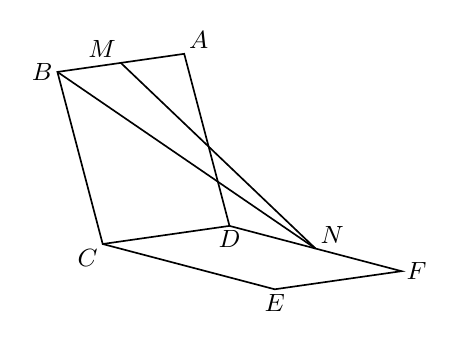
\begin{tikzpicture}[scale=1.15, semithick, every node/.style={inner sep=1.5pt, font=\small}]
  \coordinate (C) at (0.2,0);
  \coordinate (D) at (1.6,0.2);
  \coordinate (B) at (-0.3,1.9);
  \coordinate (A) at (1.1,2.1);
  \coordinate (E) at (2.1,-0.5);
  \coordinate (F) at (3.5,-0.3);
  \coordinate (M) at (0.4,2.0);
  \coordinate (N) at (2.55,-0.05);
  % 竖直正方形 ABCD
  \draw (A) -- (B) -- (C) -- (D) -- cycle;
  % 水平正方形 DCEF
  \draw (C) -- (E) -- (F) -- (D);
  % 图中线段
  \draw (M) -- (N);
  \draw (B) -- (N);
  % 顶点标注
  \node[above right] at (A) {$A$};
  \node[left] at (B) {$B$};
  \node[above left] at (M) {$M$};
  \node[below left] at (C) {$C$};
  \node[below] at (D) {$D$};
  \node[below] at (E) {$E$};
  \node[right] at (F) {$F$};
  \node[above right] at (N) {$N$};
\end{tikzpicture}
\end{center}
\nopagebreak[4]
\Needspace{4\baselineskip}
\textbf{解析}

\Needspace{5\baselineskip}
（1）以 $D$ 为原点、$DC$ 为 $x$ 轴、平面 $DCEF$ 为 $xOy$ 平面建系。由 $CD=2$、两平面垂直，可取

\nopagebreak[4]
\[D(0,0,0),\quad C(2,0,0),\quad B(2,0,2),\quad A(0,0,2),\]
\nopagebreak[4]
\[E(2,2,0),\quad F(0,2,0).\]

\Needspace{5\baselineskip}
$M$ 为 $AB$ 中点、$N$ 为 $DF$ 中点，故

\nopagebreak[4]
\[M(1,0,2),\qquad N(0,1,0),\]

\nopagebreak[4]
\[MN=\sqrt{(1-0)^2+(0-1)^2+(2-0)^2}=\sqrt6 .\]

（2）用反证法。设 $ME$ 与 $BN$ 共面，则该平面 $\alpha$ 含 $M,B,N,E$ 四点。

\Needspace{5\baselineskip}
记 $\boldsymbol e$ 为 $\overrightarrow{DC}$ 方向的单位向量，$u,v$ 分别为 $\overrightarrow{BC}$、$\overrightarrow{DE}$ 方向的单位向量。两正方形不在同一平面内，故 $u$ 与 $v$ 不平行；又都垂直于 $\boldsymbol e$，且 $|u|=|v|=1$。以 $D$ 为原点可写

\nopagebreak[4]
\[M=\boldsymbol e+2u,\quad B=2\boldsymbol e+2u,\quad E=2\boldsymbol e+2v,\quad N=v .\]

\Needspace{5\baselineskip}
于是

\nopagebreak[4]
\[\overrightarrow{MB}=\boldsymbol e,\qquad
\overrightarrow{ME}=\boldsymbol e+2(v-u),\qquad
\overrightarrow{MN}=v-\boldsymbol e-2u .\]

\Needspace{5\baselineskip}
三向量同在平面 $\alpha$ 内，故 $\overrightarrow{ME}$、$\overrightarrow{MN}$ 在垂直于 $\boldsymbol e$ 的方向上的分量必须共线，即存在实数 $\lambda$ 使

\nopagebreak[4]
\[v-2u=\lambda\cdot2(v-u)=2\lambda v-2\lambda u .\]

因 $u,v$ 不平行，比较系数得 $2\lambda=1$ 且 $2\lambda=2$，即 $\lambda=\dfrac12$ 与 $\lambda=1$ 同时成立，矛盾。

故假设不成立，$ME$ 与 $BN$ 不共面，是两条异面直线。

\gkanswer{答案：（1）$\sqrt6$；（2）证明见解析。}

\end{answer}
\begin{answer}
\gksolhead{20}{}

\textbf{题目}：

某企业有两个分厂生产某种零件，按规定内径尺寸（单位：$\mathrm{mm}$）的值落在 $[29.94,30.06]$ 的零件为优质品．从两个分厂生产的零件中个抽出 $500$ 件，量其内径尺寸，得结果如下表：
\nopagebreak[4]
\begin{center}% 2009 年辽宁卷文科第 20 题：甲、乙两分厂零件内径尺寸的频数分布表。
% 来源 PDF：普通高考/2009/2009辽宁文.pdf，SHA256 99623efa457632f26bc5d5775293bf9fd13a56add984179360e30698afc7cb73
% 原页：第 2 页（A3 三栏）第 2 栏上部，印刷页 540。
% 重绘依据：两表各 7 个分组，组距 0.04，分组与频数逐字照录原页；第三个分组原页印作
%   [29.84,29.98)（两表相同），与前后分组重叠，照录并登记问题，未擅改。
\begin{tikzpicture}[semithick, every node/.style={inner sep=2pt, font=\small}]
  % 甲厂
  \node at (1.45,0.35) {甲厂};
  \draw (0,0) rectangle (4.0,-4.55);
  \draw (2.9,0) -- (2.9,-4.55);
  \draw (0,-0.7) -- (4.0,-0.7);
  \foreach \y in {-1.25,-1.8,-2.35,-2.9,-3.45,-4.0} { \draw (0,\y) -- (4.0,\y); }
  \node at (1.45,-0.35) {分组};
  \node at (3.45,-0.35) {频数};
  \node at (1.45,-0.975) {$[29.86,\,29.90)$};
  \node at (1.45,-1.525) {$[29.90,\,29.94)$};
  \node at (1.45,-2.075) {$[29.84,\,29.98)$};
  \node at (1.45,-2.625) {$[29.98,\,30.02)$};
  \node at (1.45,-3.175) {$[30.02,\,30.06)$};
  \node at (1.45,-3.725) {$[30.06,\,30.10)$};
  \node at (1.45,-4.275) {$[30.10,\,30.14)$};
  \node at (3.45,-0.975) {$12$};
  \node at (3.45,-1.525) {$63$};
  \node at (3.45,-2.075) {$86$};
  \node at (3.45,-2.625) {$182$};
  \node at (3.45,-3.175) {$92$};
  \node at (3.45,-3.725) {$61$};
  \node at (3.45,-4.275) {$4$};
  % 乙厂
  \begin{scope}[shift={(5.2,0)}]
    \node at (1.45,0.35) {乙厂};
    \draw (0,0) rectangle (4.0,-4.55);
    \draw (2.9,0) -- (2.9,-4.55);
    \draw (0,-0.7) -- (4.0,-0.7);
    \foreach \y in {-1.25,-1.8,-2.35,-2.9,-3.45,-4.0} { \draw (0,\y) -- (4.0,\y); }
    \node at (1.45,-0.35) {分组};
    \node at (3.45,-0.35) {频数};
    \node at (1.45,-0.975) {$[29.86,\,29.90)$};
    \node at (1.45,-1.525) {$[29.90,\,29.94)$};
    \node at (1.45,-2.075) {$[29.84,\,29.98)$};
    \node at (1.45,-2.625) {$[29.98,\,30.02)$};
    \node at (1.45,-3.175) {$[30.02,\,30.06)$};
    \node at (1.45,-3.725) {$[30.06,\,30.10)$};
    \node at (1.45,-4.275) {$[30.10,\,30.14)$};
    \node at (3.45,-0.975) {$29$};
    \node at (3.45,-1.525) {$71$};
    \node at (3.45,-2.075) {$85$};
    \node at (3.45,-2.625) {$159$};
    \node at (3.45,-3.175) {$76$};
    \node at (3.45,-3.725) {$62$};
    \node at (3.45,-4.275) {$18$};
  \end{scope}
\end{tikzpicture}
\end{center}
\nopagebreak[4]
（1）试分别估计两个分厂生产的零件的优质品率；

（2）由于以上统计数据填下面 $2\times2$ 列联表，并问是否有 $99\%$ 的把握认为「两个分厂生产的零件的质量有差异」．
\nopagebreak[4]
\begin{center}% 2009 年辽宁卷文科第 20 题：2×2 列联表（待填）。
% 来源 PDF：普通高考/2009/2009辽宁文.pdf，SHA256 99623efa457632f26bc5d5775293bf9fd13a56add984179360e30698afc7cb73
% 原页：第 2 页（A3 三栏）第 2 栏中部，印刷页 540。
% 重绘依据：行标签为优质品、非优质品、合计，列标签为甲厂、乙厂、合计；表内单元格在原页留空，待填。
\begin{tikzpicture}[semithick, every node/.style={inner sep=2pt, font=\small}]
  \draw (0,0) rectangle (7.4,-2.8);
  \draw (2.6,0) -- (2.6,-2.8);
  \draw (4.2,0) -- (4.2,-2.8);
  \draw (5.8,0) -- (5.8,-2.8);
  \foreach \y in {-0.7,-1.4,-2.1} { \draw (0,\y) -- (7.4,\y); }
  \node at (1.3,-0.35) {};
  \node at (3.4,-0.35) {甲厂};
  \node at (5.0,-0.35) {乙厂};
  \node at (6.6,-0.35) {合计};
  \node at (1.3,-1.05) {优质品};
  \node at (1.3,-1.75) {非优质品};
  \node at (1.3,-2.45) {合计};
\end{tikzpicture}
\end{center}
\nopagebreak[4]
\Needspace{10\baselineskip}
附：$\chi^2=\frac{n(n_{11}n_{22}-n_{12}n_{21})^2}{n_{1+}n_{2+}n_{+1}n_{+2}}$，

\begin{center}
\begin{tabular}{lll}
\toprule
$P(\chi^2\geqslant k)$ & $0.05$ & $0.01$ \\
\midrule
$k$ & $3.841$ & $6.635$ \\
\bottomrule
\end{tabular}
\end{center}

\Needspace{4\baselineskip}
\textbf{解析}

（1）优质品是内径落在 $[29.94,30.06]$ 的零件。原页第三个分组印作 $[29.84,29.98)$，按组距 $0.04$ 与前后分组首尾相接，应为 $[29.94,29.98)$，故取第三、四、五组。

\Needspace{5\baselineskip}
甲厂优质品频率为

\nopagebreak[4]
\[\frac{86+182+92}{500}=\frac{360}{500}=0.72,\]

\Needspace{5\baselineskip}
乙厂优质品频率为

\nopagebreak[4]
\[\frac{85+159+76}{500}=\frac{320}{500}=0.64 .\]

（2）按优质品与非优质品整理成列联表：

\begin{center}
\begin{tabular}{llll}
\toprule
 & 甲厂 & 乙厂 & 合计 \\
\midrule
优质品 & $360$ & $320$ & $680$ \\
非优质品 & $140$ & $180$ & $320$ \\
合计 & $500$ & $500$ & $1000$ \\
\bottomrule
\end{tabular}
\end{center}

\Needspace{5\baselineskip}
代入公式：

\nopagebreak[4]
\[\chi^2=\frac{1000(360\times180-320\times140)^2}{680\times320\times500\times500}
=\frac{1000\times20000^2}{680\times320\times500\times500}\approx7.35 .\]

因 $7.35>6.635$，故有 $99\%$ 的把握认为两个分厂生产的零件质量有差异。

\gkanswer{答案：（1）甲厂 $72\%$，乙厂 $64\%$；（2）$\chi^2\approx7.35>6.635$，有 $99\%$ 的把握。}

\end{answer}
\begin{answer}
\gksolhead{21}{}

\textbf{题目}：

设 $f(x)=\mathrm e^x(ax^2+x+1)$，且曲线 $y=f(x)$ 在 $x=1$ 处的切线与 $x$ 轴平行．

（1）求 $a$ 的值，并讨论 $f(x)$ 的单调性；

（2）证明：当 $\theta\in\left[0,\frac\pi2\right]$ 时，$|f(\cos\theta)-f(\sin\theta)|<2$．

\Needspace{4\baselineskip}
\textbf{解析}

\Needspace{5\baselineskip}
（1）求导：

\nopagebreak[4]
\[f'(x)=\mathrm e^x(ax^2+x+1)+\mathrm e^x(2ax+1)
=\mathrm e^x\left[ax^2+(2a+1)x+2\right].\]

\Needspace{5\baselineskip}
曲线在 $x=1$ 处的切线与 $x$ 轴平行，故 $f'(1)=0$：

\nopagebreak[4]
\[\mathrm e\left[a+(2a+1)+2\right]=0\ \Longrightarrow\ 3a+3=0\ \Longrightarrow\ a=-1 .\]

\Needspace{5\baselineskip}
此时

\nopagebreak[4]
\[f'(x)=\mathrm e^x(-x^2-x+2)=-\mathrm e^x(x+2)(x-1).\]

$f'(x)<0$ 当 $x<-2$ 或 $x>1$；$f'(x)>0$ 当 $-2<x<1$。故 $f(x)$ 在 $(-2,1)$ 上单调递增，在 $(-\infty,-2)$ 与 $(1,+\infty)$ 上单调递减。

\Needspace{5\baselineskip}
（2）当 $\theta\in\left[0,\dfrac\pi2\right]$ 时，$\cos\theta,\sin\theta\in[0,1]$。由（1），$f$ 在 $[0,1]$ 上单调递增，故对一切 $t\in[0,1]$，

\nopagebreak[4]
\[f(0)\leqslant f(t)\leqslant f(1).\]

\Needspace{5\baselineskip}
由 $f(0)=\mathrm e^0(0+0+1)=1$，$f(1)=\mathrm e(-1+1+1)=\mathrm e$，得

\nopagebreak[4]
\[|f(\cos\theta)-f(\sin\theta)|\leqslant f(1)-f(0)=\mathrm e-1<2 .\]

于是所证不等式成立。

\gkanswer{答案：（1）$a=-1$；$f(x)$ 在 $(-2,1)$ 上单调递增，在 $(-\infty,-2)$ 与 $(1,+\infty)$ 上单调递减；（2）证明见解析。}

\end{answer}
\begin{answer}
\gksolhead{22}{}

\textbf{题目}：

已知椭圆 $C$ 过点 $A\left(1,\frac32\right)$，两个焦点为 $(-1,0)$，$(1,0)$．

（1）求椭圆 $C$ 的方程；

（2）$E,F$ 是椭圆 $C$ 上的两个动点，如果直线 $AE$ 的斜率与 $AF$ 的斜率互为相反数，证明直线 $EF$ 的斜率为定值，并求出这个定值．

\Needspace{4\baselineskip}
\textbf{解析}

\Needspace{5\baselineskip}
（1）设椭圆方程为 $\dfrac{x^2}{a^2}+\dfrac{y^2}{b^2}=1$（$a>b>0$）。焦点为 $(\pm1,0)$，故 $c=1$，$a^2=b^2+1$。代入 $A\left(1,\dfrac32\right)$：

\nopagebreak[4]
\[\frac{1}{b^2+1}+\frac{9}{4b^2}=1 .\]

\Needspace{5\baselineskip}
两边乘以 $4b^2(b^2+1)$：

\nopagebreak[4]
\[4b^2+9(b^2+1)=4b^2(b^2+1)
\ \Longrightarrow\ 4b^4-9b^2-9=0
\ \Longrightarrow\ b^2=3\ \text{\text{或}}\ b^2=-\frac34,\]

\Needspace{5\baselineskip}
取 $b^2=3$，则 $a^2=4$，椭圆为

\nopagebreak[4]
\[\frac{x^2}{4}+\frac{y^2}{3}=1 .\]

\Needspace{5\baselineskip}
（2）设 $AE$ 的斜率为 $k$，则 $AF$ 的斜率为 $-k$。过 $A$ 的直线 $AE$：

\nopagebreak[4]
\[y=k(x-1)+\frac32=kx+\left(\frac32-k\right).\]

\Needspace{5\baselineskip}
记 $m=\dfrac32-k$，代入 $3x^2+4y^2=12$：

\nopagebreak[4]
\[(3+4k^2)x^2+8kmx+4m^2-12=0 .\]

\Needspace{5\baselineskip}
$x=1$ 是一个根（点 $A$），由韦达定理，另一根为

\nopagebreak[4]
\[x_E=\frac{4m^2-12}{3+4k^2}=\frac{4k^2-12k-3}{3+4k^2},\]

其中用到 $4\left(\dfrac32-k\right)^2-12=4k^2-12k-3$。

\Needspace{5\baselineskip}
把 $k$ 换成 $-k$ 得

\nopagebreak[4]
\[x_F=\frac{4k^2+12k-3}{3+4k^2}.\]

\Needspace{5\baselineskip}
于是

\nopagebreak[4]
\[x_E+x_F=\frac{8k^2-6}{3+4k^2},\qquad
x_E-x_F=\frac{-24k}{3+4k^2}.\]

\Needspace{5\baselineskip}
又 $y_E=kx_E+m$，$y_F=-kx_F+\left(\dfrac32+k\right)$，故

\nopagebreak[4]
\[y_E-y_F=k(x_E+x_F)-2k
=\frac{k(8k^2-6)-2k(3+4k^2)}{3+4k^2}
=\frac{-12k}{3+4k^2}.\]

\Needspace{5\baselineskip}
所以

\nopagebreak[4]
\[k_{EF}=\frac{y_E-y_F}{x_E-x_F}
=\frac{-12k}{3+4k^2}\cdot\frac{3+4k^2}{-24k}=\frac12,\]

即直线 $EF$ 的斜率为定值 $\dfrac12$。

\gkanswer{答案：（1）$\frac{x^2}{4}+\frac{y^2}{3}=1$；（2）定值为 $\frac12$。}

\end{answer}